% !TeX root = ../main.tex
% Add the above to each chapter to make compiling the PDF easier in some editors.

\chapter{Foundations}\label{chapter:foundations}

\section{L4 Fiasco.OC}
The ECU infrastructure described in the KIA4SM project is mainly composed of microcontrollers, on which microkernels are used. The concept of such a microkernel is that only the minimal base functionality should reside within the kernel, while all other functionalities are considered user space and therefore handled by the operating system above. Because of this superior software technology compared to monolithic kernels such as Linux, without inherent loss of performance or flexibility \cite{micro}, they provide a perfect fit for embedded distributed systems.

Fiasco.OC, also known as L4Re Microkernel is the specific microkernel chosen for this project. It provides features essential for KIA4SM and RTCR such as hardware assisted virtualisation, multi-processor support and real-time scheduling. Also its features make it fit well within the Genode paradigm, with an object-oriented capability system and kernel resource control \cite{fiasco}. Therefore, this kernel was the choice for the original build of RTCR, and the decision of which microkernel to use for the CMS was made in favour of Fiasco.OC, too.

\section{Genode Operating System Framework}
The Genode OS framework is a tool kit for building special-purpose operating systems with the ability to support small embedded systems all the way up to highly dynamic general-purpose workloads. Furthermore, the foundation for a focus on high security is laid by the architecture of Genode, which is presented in the following sections. \cite[P.14]{genode_foundations}
\subsection{Capability-based security}
One main aspect of Genode is that its architecture is object oriented, providing a layer of abstraction, assisting with designing and understanding. A process inside this architecture is called a component, which has its own protection domain that defines process boundaries. Initially, it is therefore impossible for another component without the correct rights to access any objects within this protection domain. These access rights are termed capabilities, around which the internal security is built, and the corresponding objects are called RPC objects. These objects provide a remote-procedure call (RPC) interface, and a capability to them, is what a pointer is to a regular object in C or C++.

A component has a capability for every RPC object within its protection domain. To prevent forging of such capabilities, and for the kernel to know which component owns such capabilities, a capability space resides within the kernel space. This capability space is represented as an array of object identities, which are generated at creation-time of the corresponding RPC objects. The capability itself then indexes the matching object identity. This relationship is displayed in figure \ref{fig:Cap_space}. \cite[P.40-41]{genode_foundations}
\begin{figure}
    \centering
    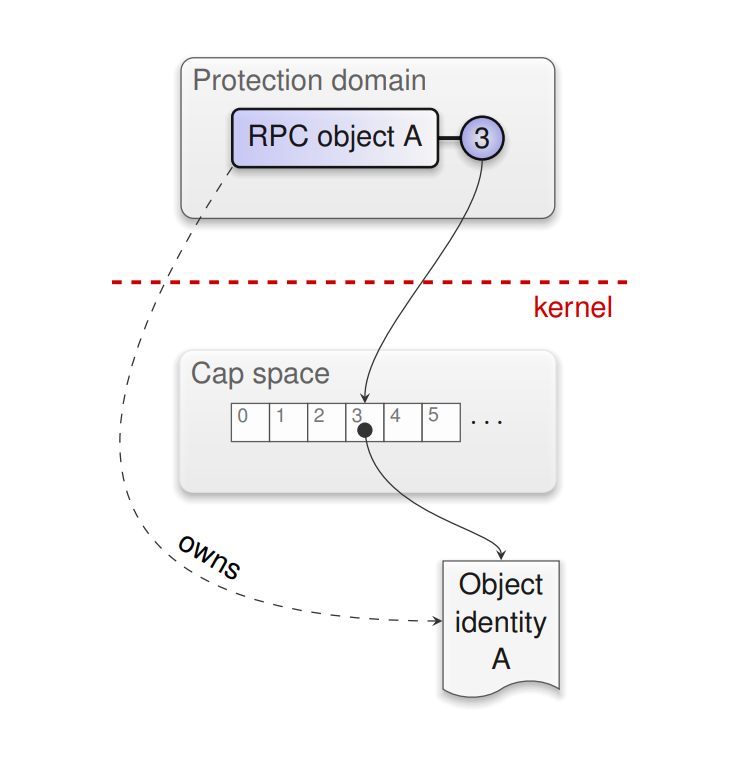
\includegraphics[width=0.5\textwidth]{Images/Cap_space.PNG}
    \caption{Relationship between an RPC object and its corresponding object identity. \cite[P.41]{genode_foundations}}
    \label{fig:Cap_space}
\end{figure}
\subsubsection{Capability Delegation}
Finally the question of how RPC objects can be accessed from other components remains. This is solved by sharing capabilities through the concept of delegation. Similarly to aforementioned pointer, a capability can be passed to another component, with which the associated RPC object can then be evoked. These delegated capabilities each index an element in the capability space of the component it was delegated to, but these elements in turn point to the same object identity. The concept of delegation, which is illustrated in figure \ref{fig:delegation}, is essential for purposes of any inter-component communication, and therefore represents a backbone of the entire architecture. \cite[P.41-42]{genode_foundations}
\begin{figure}
    \centering
    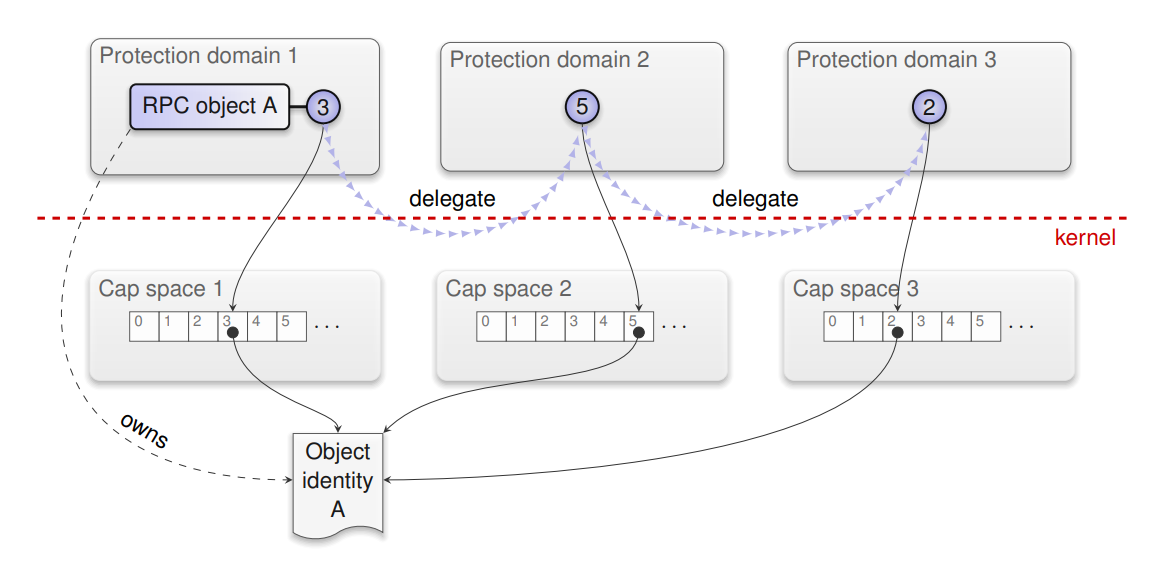
\includegraphics[width=0.75\textwidth]{Images/delegation.PNG}
    \caption{The transitive delegation of a capability from one protection domain to others. \cite[P.42]{genode_foundations}}
    \label{fig:delegation}
\end{figure}
\subsection{Recursive System Structure}
The last section introduced the fundamental parts of the Genode architecture, but what remains to be explained is how these components are connected to each other. The overall system structure is a tree of components, where every component except the root of this tree has a parent. This root is called core and it has access to the raw physical resources, which it then distributes to other components as capabilities to RPC objects. These RPC objects that interface the physical resources are:
\begin{itemize}
    \item Dataspaces: A dataspace is the representation of a physical address-space region of any size.
    \item Region maps: A region map is the layout of a virtual address space. Similarly to how a MMU populates page tables with physical page frames, a region map is populated with dataspaces. One dataspace can therefore be attached to multiple region maps.
    \item Access to boot modules (ROM): These RPC objects represent different binaries initially loaded into the memory by the boot loader, which are then made available as read-only memory to clients. 
    \item Protection domains (PD): A protection domain defines the boundaries of a component within the Genode system, where typically one PD corresponds to one component. Each PD consists of three region maps, a capability space, and a physical memory and capability budget.
    \item Region-map management (RM): The RM service allows components to allocate more than the aforementioned three region maps.
    \item Processing-time allocation (CPU): The CPU service can be used to create, control and terminate threads.
    \item "Device resources (IO\_MEM, IO\_PORT, IRQ): Core’s IO\_MEM, IO\_PORT, and IRQ services enable the realization of user-level device drivers as Genode components." \cite[P.69]{genode_foundations}
    \item Logging (LOG): The LOG service allows components to print diagnostic output.
    \item Event tracing (TRACE): The TRACE service is a non-fundamental light-weight event-tracing facility.
\end{itemize}
\cite[P.65-71]{genode_foundations}

\subsubsection{Client-Server Relationship}
To now establish a connection between a component offering a service (server) and another component that wants to use this service (client), a multitude of actions have to be performed. This is explained using the example of a GUI component as a server, offering a GUI service, and an application, which represents the client. Firstly, the GUI component has to announce its service to its parent using its parent interface, which is a capability to the parent RPC object that was delegated to it at creation time. Announcing is done by delegating a capability to the service root RPC object. 

On the other side, the application requests a GUI session from its parent interface. These requests are passed up the tree until it reaches the parent of the GUI component, which uses its capability to the root RPC object to create a session RPC object. A capability to that session RPC object is then passed to the initial caller. Figure \ref{fig:client-server} shows the setup after the final delegation was made. 

It is important to highlight that due to the parent having complete control over both the sessions established within the child on server side and requests done by the child on client side, security is further improved. \cite[P.50-54]{genode_foundations}
\begin{figure}
    \centering
    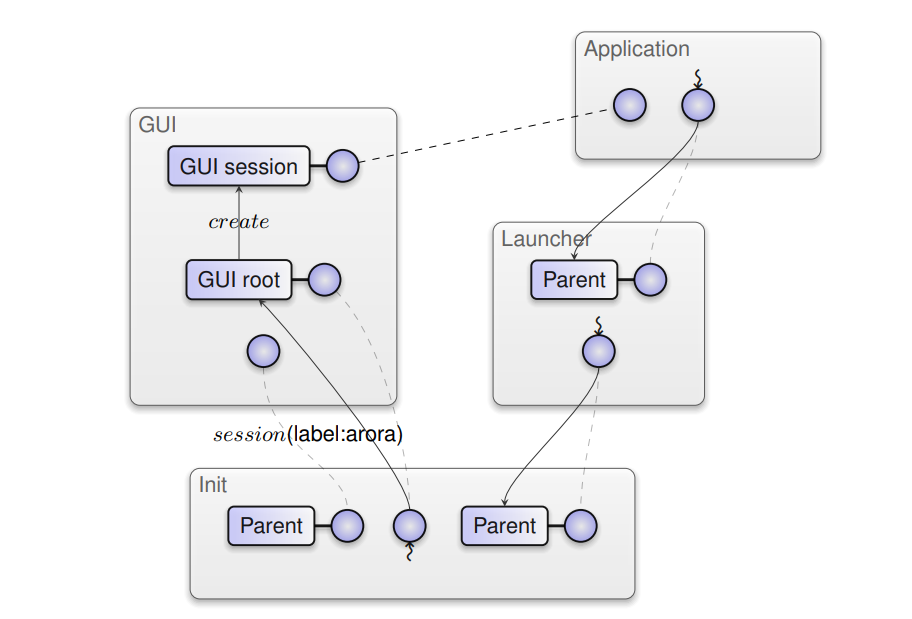
\includegraphics[width=0.75\textwidth]{Images/client-server.PNG}
    \caption{Example of client-server relationship after final session delegation. \cite[P.52]{genode_foundations}}
    \label{fig:client-server}
\end{figure}
\newline
\newline
Within an actual project, a session interface defining the RPC functions needs to be created as the first step. This interface is implemented inside a session component object by the server, which can be created by the server's parent because the servers root component was announced to it, handing it the capability. 

To implement a complete client, a session client class which takes a session capability in its constructor and implements the RPC interface for the client, has to be declared. The remaining issue now is how a session client object would obtain the necessary capability. The solution being a wrapper called a connection object, which inherits from the session client. This object is responsible for issuing a session request to the parent and retrieving the capability, with which a session client object can be created. Because of this preparatory work the client side implementation is straightforward: it simply declares a connection corresponding to the service that it wants to use and calls functions on it as if it were a session client object. A simplified illustration of the classes making up this functionality can be seen in figure \ref{fig:client-server_classdiagram}. \cite{client-server_tutorial}
\begin{figure}
    \centering
    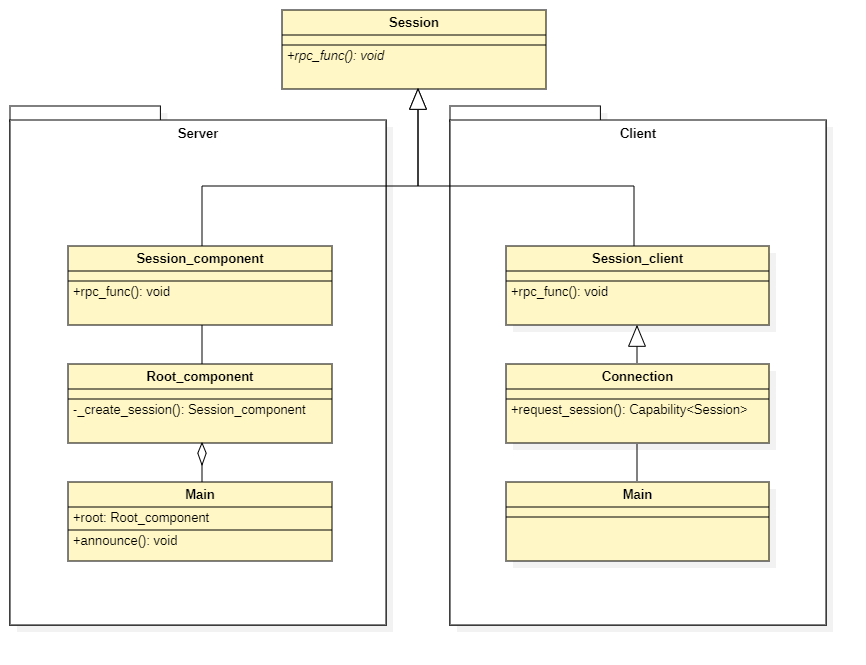
\includegraphics[width=0.7\textwidth]{Images/client-server_classdiagram.png}
    \caption{Class diagram of the components making up the client-server infrastructure.}
    \label{fig:client-server_classdiagram}
\end{figure}

\subsection{Networking in the Genode OS framework}\label{subsection:network}
Since the checkpoint management system has to be able to communicate with other components across ECU boundaries, the network stack comes into play. In Genode, most user-level network communication is done using the socket API, which is handled by a lightweight TCP/IP stack called lwIP. The network stacks of the different components then access a network interface controller session provided by a NIC-router, which acts as a multiplexing component so that the applications do not directly operate on the actual network drivers, allowing the use of the networking interface by multiple applications.

Instead of having the NIC-driver delegate a session to the NIC-router, as was generally the case until Genode version 21.02, the driver acts as a client towards the router by using a so-called uplink session, provided by the latter. This architectural change was implemented because the NIC driver was deemed too fragile due to its high complexity, leading to the lifetime of an application being put at risk by being bound to it. The structure is depicted in figure \ref{fig:network_architecture} with the additional underlying components of platform driver, core/init, and the kernel. \cite{nic}

\begin{figure}
    \centering
    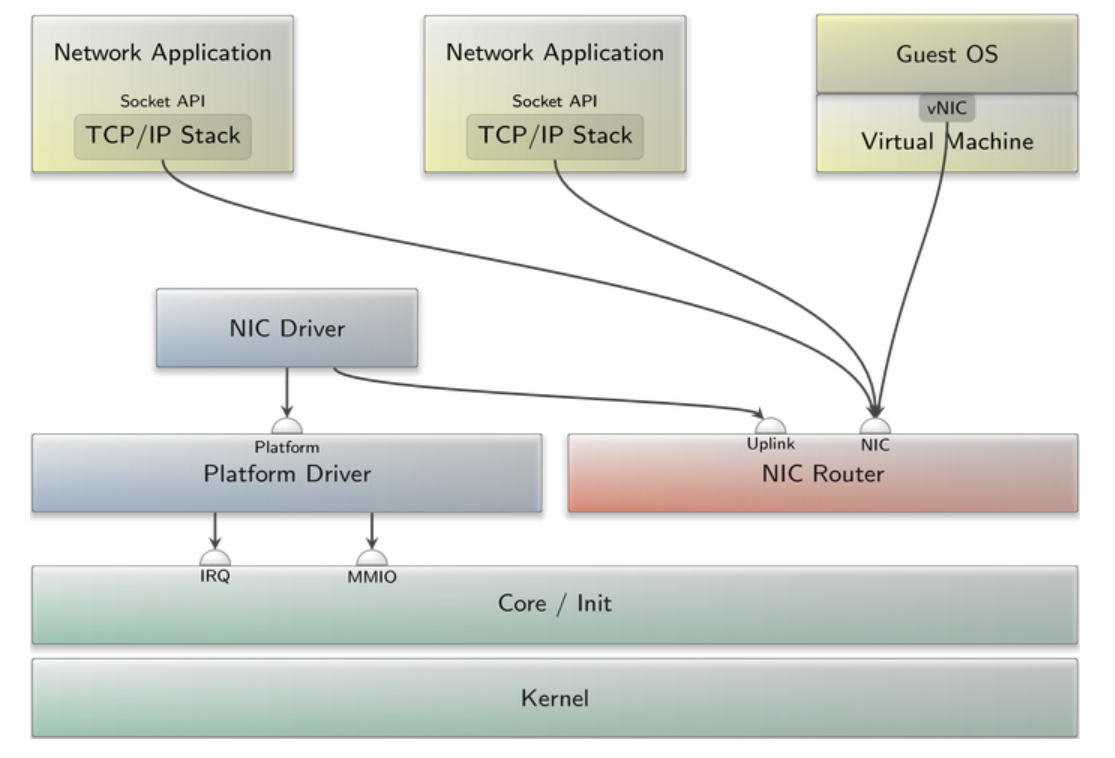
\includegraphics[width=0.7\textwidth]{Images/network_architecture.png}
    \caption{Visualisation of the Genode OS network architecture after Genode 21.02. \cite{nic}}
    \label{fig:network_architecture}
\end{figure}

\section{Distributed Shared Memory for Genode}\label{section:DSM}
The development of a checkpoint management system necessitates data transfer between components running on different ECUs. One way to accomplish this and possibly answer the research question regarding receipt of checkpoints is by a distributed shared memory (DSM), of which a prototype was developed by Weidinger in 2016 for Fiasco.OC/Genode OS 15.02.

The main functionality of establishing and updating the shared memory is handled by two broker components which are spawned by the processes that wish to share memory across system boundaries. These brokers first establish a local shared memory by delegating a capability to the dataspace and then detect read and write accesses to the memory on their respective sides by the handling of page faults, which triggers the sending of data to the other system over Ethernet using TCP/IP. It is important to note that because of the local shared memory, the DSM functionality is completely transparent to both processes. 

However, the consistency module, which checks if both dataspaces representing the shared memory are identical and is an essential aspect of an DSM is not implemented. \cite{dsm}